%  LaTeX support: latex@mdpi.com 
%DIF LATEXDIFF DIFFERENCE FILE
%DIF DEL paper.tex     Tue May 30 15:22:23 2023
%DIF ADD paperv1.tex   Tue Jun 13 23:17:20 2023
%  For support, please attach all files needed for compiling as well as the log file, and specify your operating system, LaTeX version, and LaTeX editor.

%=================================================================
\documentclass[mathematics,article,submit,moreauthors]{Definitions/mdpi} 

%--------------------
% Class Options:
%--------------------
%----------
% journal
%----------
% Choose between the following MDPI journals:
% acoustics, actuators, addictions, admsci, adolescents, aerobiology, aerospace, agriculture, agriengineering, agrochemicals, agronomy, ai, air, algorithms, allergies, alloys, analytica, analytics, anatomia, animals, antibiotics, antibodies, antioxidants, applbiosci, appliedchem, appliedmath, applmech, applmicrobiol, applnano, applsci, aquacj, architecture, arm, arthropoda, arts, asc, asi, astronomy, atmosphere, atoms, audiolres, automation, axioms, bacteria, batteries, bdcc, behavsci, beverages, biochem, bioengineering, biologics, biology, biomass, biomechanics, biomed, biomedicines, biomedinformatics, biomimetics, biomolecules, biophysica, biosensors, biotech, birds, bloods, blsf, brainsci, breath, buildings, businesses, cancers, carbon, cardiogenetics, catalysts, cells, ceramics, challenges, chemengineering, chemistry, chemosensors, chemproc, children, chips, cimb, civileng, cleantechnol, climate, clinpract, clockssleep, cmd, coasts, coatings, colloids, colorants, commodities, compounds, computation, computers, condensedmatter, conservation, constrmater, cosmetics, covid, crops, cryptography, crystals, csmf, ctn, curroncol, cyber, dairy, data, ddc, dentistry, dermato, dermatopathology, designs, devices, diabetology, diagnostics, dietetics, digital, disabilities, diseases, diversity, dna, drones, dynamics, earth, ebj, ecologies, econometrics, economies, education, ejihpe, electricity, electrochem, electronicmat, electronics, encyclopedia, endocrines, energies, eng, engproc, entomology, entropy, environments, environsciproc, epidemiologia, epigenomes, est, fermentation, fibers, fintech, fire, fishes, fluids, foods, forecasting, forensicsci, forests, foundations, fractalfract, fuels, future, futureinternet, futurepharmacol, futurephys, futuretransp, galaxies, games, gases, gastroent, gastrointestdisord, gels, genealogy, genes, geographies, geohazards, geomatics, geosciences, geotechnics, geriatrics, grasses, gucdd, hazardousmatters, healthcare, hearts, hemato, hematolrep, heritage, higheredu, highthroughput, histories, horticulturae, hospitals, humanities, humans, hydrobiology, hydrogen, hydrology, hygiene, idr, ijerph, ijfs, ijgi, ijms, ijns, ijpb, ijtm, ijtpp, ime, immuno, informatics, information, infrastructures, inorganics, insects, instruments, inventions, iot, j, jal, jcdd, jcm, jcp, jcs, jcto, jdb, jeta, jfb, jfmk, jimaging, jintelligence, jlpea, jmmp, jmp, jmse, jne, jnt, jof, joitmc, jor, journalmedia, jox, jpm, jrfm, jsan, jtaer, jvd, jzbg, kidneydial, kinasesphosphatases, knowledge, land, languages, laws, life, liquids, literature, livers, logics, logistics, lubricants, lymphatics, machines, macromol, magnetism, magnetochemistry, make, marinedrugs, materials, materproc, mathematics, mca, measurements, medicina, medicines, medsci, membranes, merits, metabolites, metals, meteorology, methane, metrology, micro, microarrays, microbiolres, micromachines, microorganisms, microplastics, minerals, mining, modelling, molbank, molecules, mps, msf, mti, muscles, nanoenergyadv, nanomanufacturing,\gdef\@continuouspages{yes}} nanomaterials, ncrna, ndt, network, neuroglia, neurolint, neurosci, nitrogen, notspecified, %%nri, nursrep, nutraceuticals, nutrients, obesities, oceans, ohbm, onco, %oncopathology, optics, oral, organics, organoids, osteology, oxygen, parasites, parasitologia, particles, pathogens, pathophysiology, pediatrrep, pharmaceuticals, pharmaceutics, pharmacoepidemiology,\gdef\@ISSN{2813-0618}\gdef\@continuous pharmacy, philosophies, photochem, photonics, phycology, physchem, physics, physiologia, plants, plasma, platforms, pollutants, polymers, polysaccharides, poultry, powders, preprints, proceedings, processes, prosthesis, proteomes, psf, psych, psychiatryint, psychoactives, publications, quantumrep, quaternary, qubs, radiation, reactions, receptors, recycling, regeneration, religions, remotesensing, reports, reprodmed, resources, rheumato, risks, robotics, ruminants, safety, sci, scipharm, sclerosis, seeds, sensors, separations, sexes, signals, sinusitis, skins, smartcities, sna, societies, socsci, software, soilsystems, solar, solids, spectroscj, sports, standards, stats, std, stresses, surfaces, surgeries, suschem, sustainability, symmetry, synbio, systems, targets, taxonomy, technologies, telecom, test, textiles, thalassrep, thermo, tomography, tourismhosp, toxics, toxins, transplantology, transportation, traumacare, traumas, tropicalmed, universe, urbansci, uro, vaccines, vehicles, venereology, vetsci, vibration, virtualworlds, viruses, vision, waste, water, wem, wevj, wind, women, world, youth, zoonoticdis 
% For posting an early version of this manuscript as a preprint, you may use "preprints" as the journal. Changing "submit" to "accept" before posting will remove line numbers.

%---------
% article
%---------
% The default type of manuscript is "article", but can be replaced by: 
% abstract, addendum, article, book, bookreview, briefreport, casereport, comment, commentary, communication, conferenceproceedings, correction, conferencereport, entry, expressionofconcern, extendedabstract, datadescriptor, editorial, essay, erratum, hypothesis, interestingimage, obituary, opinion, projectreport, reply, retraction, review, perspective, protocol, shortnote, studyprotocol, systematicreview, supfile, technicalnote, viewpoint, guidelines, registeredreport, tutorial
% supfile = supplementary materials

%----------
% submit
%----------
% The class option "submit" will be changed to "accept" by the Editorial Office when the paper is accepted. This will only make changes to the frontpage (e.g., the logo of the journal will get visible), the headings, and the copyright information. Also, line numbering will be removed. Journal info and pagination for accepted papers will also be assigned by the Editorial Office.

%------------------
% moreauthors
%------------------
% If there is only one author the class option oneauthor should be used. Otherwise use the class option moreauthors.

%---------
% pdftex
%---------
% The option pdftex is for use with pdfLaTeX. Remove "pdftex" for (1) compiling with LaTeX & dvi2pdf (if eps figures are used) or for (2) compiling with XeLaTeX.

%=================================================================
% MDPI internal commands - do not modify
\firstpage{1} 
\makeatletter 
\setcounter{page}{\@firstpage} 
\makeatother
\pubvolume{1}
\issuenum{1}
\articlenumber{0}
\pubyear{2023}
\copyrightyear{2023}
%\externaleditor{Academic Editor: Firstname Lastname}
\datereceived{ } 
\daterevised{ } % Comment out if no revised date
\dateaccepted{ } 
\datepublished{ } 
%\datecorrected{} % For corrected papers: "Corrected: XXX" date in the original paper.
%\dateretracted{} % For corrected papers: "Retracted: XXX" date in the original paper.
\hreflink{https://doi.org/} % If needed use \linebreak
%\doinum{}
%\pdfoutput=1 % Uncommented for upload to arXiv.org

%=================================================================
% Add packages and commands here. The following packages are loaded in our class file: fontenc, inputenc, calc, indentfirst, fancyhdr, graphicx, epstopdf, lastpage, ifthen, float, amsmath, amssymb, lineno, setspace, enumitem, mathpazo, booktabs, titlesec, etoolbox, tabto, xcolor, colortbl, soul, multirow, microtype, tikz, totcount, changepage, attrib, upgreek, array, tabularx, pbox, ragged2e, tocloft, marginnote, marginfix, enotez, amsthm, natbib, hyperref, cleveref, scrextend, url, geometry, newfloat, caption, draftwatermark, seqsplit
% cleveref: load \crefname definitions after \begin{document}

%=================================================================
% Please use the following mathematics environments: Theorem, Lemma, Corollary, Proposition, Characterization, Property, Problem, Example, ExamplesandDefinitions, Hypothesis, Remark, Definition, Notation, Assumption
%% For proofs, please use the proof environment (the amsthm package is loaded by the MDPI class).

%=================================================================
% Full title of the paper (Capitalized)
\Title{Multitask Fine-tuning on Pretrained Language Model for Retrieval-based Question Answering in Automotive Domain}

% MDPI internal command: Title for citation in the left column
\TitleCitation{Title}

% Author Orchid ID: enter ID or remove command
\newcommand{\orcidauthorA}{0000-0002-2206-1926} % Add \orcidA{} behind the author's name
%\newcommand{\orcidauthorB}{0000-0000-0000-000X} % Add \orcidB{} behind the author's name

% Authors, for the paper (add full first names)
\Author{Zhiyi Luo $^{1}$\orcidA{}, Sirui Yan $^{1}$ and Shuyun Luo $^{1,}$*}

%\longauthorlist{yes}

% MDPI internal command: Authors, for metadata in PDF
\AuthorNames{Zhiyi Luo, Sirui Yan and Shuyun Luo}

% MDPI internal command: Authors, for citation in the left column
\AuthorCitation{Luo, Z.; Yan, S.; Luo, S.}
% If this is a Chicago style journal: Lastname, Firstname, Firstname Lastname, and Firstname Lastname.

% Affiliations / Addresses (Add [1] after \address if there is only one affiliation.)
\address{%
$^{1}$ \quad School of Computer Science and Technology, Zhejiang Sci-Tech University, Hangzhou, China; luozhiyi@zstu.edu.cn
%$^{2}$ \quad Affiliation 2; e-mail@e-mail.com
}

% Contact information of the corresponding author
\corres{Correspondence: shuyunluo@zstu.edu.cn;}

% Current address and/or shared authorship
%\firstnote{Current address: Affiliation 3.} 
%\secondnote{These authors contributed equally to this work.}
% The commands \thirdnote{} till \eighthnote{} are available for further notes

%\simplesumm{} % Simple summary

%\conference{} % An extended version of a conference paper

% Abstract (Do not insert blank lines, i.e. \\) 
%DIF 111c111
%DIF < \abstract{Retrieval-based question answering in the automotive domain requires a model to comprehend and articulate relevant domain knowledge, accurately understand user intent, and effectively match the required information. Typically, these systems employ a encoder-retriever architecture. However, existing encoders, which rely on pretrained language models, suffer from limited specialization, insufficient awareness of domain knowledge, and biases in user intent understanding. To overcome these limitations, this paper constructs a Chinese corpus specifically tailored for the automotive domain, comprising question-answer pairs, document collections, and multitask annotated data. Subsequently, a pretraining-multitask fine-tuning framework based on masked language models is introduced to integrate domain knowledge as well as enhance semantic representations, thereby yielding benefits for downstream applications. To evaluate system performance, an evaluation dataset is created using ChatGPT, and a novel retrieval task evaluation metric called Mean Linear Window Rank (MLWR) is proposed. Experimental results demonstrate that the proposed system achieves accuracies of 77.5\% and 84.75\% for Hit@1 and Hit@3 respectively, in the automotive domain retrieval-based question answering task. Additionally, the MLWR reaches 87.71\%. Compared to a system utilizing a general encoder, the proposed multitask fine-tuning strategy shows improvements of 12.5\%, 12.5\%, and 28.16\% for Hit@1, Hit@3, and MLWR, respectively. Furthermore, when compared to the best single-task fine-tuning strategy, the enhancements amount to 0.5\%, 1.25\%, and 0.95\% for Hit@1, Hit@3, and MLWR, respectively.}
%DIF -------
\abstract{Retrieval-based question answering in the automotive domain requires a model to comprehend and articulate relevant domain knowledge, accurately understand user intent, and effectively match the required information. Typically, these systems employ a encoder-retriever architecture. However, existing encoders, which rely on pretrained language models, suffer from limited specialization, insufficient awareness of domain knowledge, and biases in user intent understanding. To overcome these limitations, this paper constructs a Chinese corpus specifically tailored for the automotive domain, comprising question-answer pairs, document collections, and multitask annotated data. Subsequently, a pretraining-multitask fine-tuning framework based on masked language models is introduced to integrate domain knowledge as well as enhance semantic representations, thereby yielding benefits for downstream applications. To evaluate system performance, an evaluation dataset is created using ChatGPT, and a novel retrieval task evaluation metric called Mean Linear Window Rank (MLWR) is proposed. Experimental results demonstrate that the proposed system (based on $\text{BERT}_{base}$), achieves accuracies of 77.5\% and 84.75\% for Hit@1 and Hit@3 respectively, in the automotive domain retrieval-based question answering task. Additionally, the MLWR reaches 87.71\%. Compared to a system utilizing a general encoder, the proposed multitask fine-tuning strategy shows improvements of 12.5\%, 12.5\%, and 28.16\% for Hit@1, Hit@3, and MLWR, respectively. Furthermore, when compared to the best single-task fine-tuning strategy, the enhancements amount to 0.5\%, 1.25\%, and 0.95\% for Hit@1, Hit@3, and MLWR, respectively.} %DIF > 
%DIF -------

% Keywords
\keyword{deep learning; pretrained language model; retrieval-based question answering; multitask learning; fine-tuning} 

% The fields PACS, MSC, and JEL may be left empty or commented out if not applicable
%\PACS{J0101}
%\MSC{}
%\JEL{}

%%%%%%%%%%%%%%%%%%%%%%%%%%%%%%%%%%%%%%%%%%
% Only for the journal Diversity
%\LSID{\url{http://}}

%%%%%%%%%%%%%%%%%%%%%%%%%%%%%%%%%%%%%%%%%%
% Only for the journal Applied Sciences
%\featuredapplication{Authors are encouraged to provide a concise description of the specific application or a potential application of the work. This section is not mandatory.}
%%%%%%%%%%%%%%%%%%%%%%%%%%%%%%%%%%%%%%%%%%

%%%%%%%%%%%%%%%%%%%%%%%%%%%%%%%%%%%%%%%%%%
% Only for the journal Data
%\dataset{DOI number or link to the deposited data set if the data set is published separately. If the data set shall be published as a supplement to this paper, this field will be filled by the journal editors. In this case, please submit the data set as a supplement.}
%\datasetlicense{License under which the data set is made available (CC0, CC-BY, CC-BY-SA, CC-BY-NC, etc.)}

%%%%%%%%%%%%%%%%%%%%%%%%%%%%%%%%%%%%%%%%%%
% Only for the journal Toxins
%\keycontribution{The breakthroughs or highlights of the manuscript. Authors can write one or two sentences to describe the most important part of the paper.}

%%%%%%%%%%%%%%%%%%%%%%%%%%%%%%%%%%%%%%%%%%
% Only for the journal Encyclopedia
%\encyclopediadef{For entry manuscripts only: please provide a brief overview of the entry title instead of an abstract.}

%%%%%%%%%%%%%%%%%%%%%%%%%%%%%%%%%%%%%%%%%%
% Only for the journal Advances in Respiratory Medicine
%\addhighlights{yes}
%\renewcommand{\addhighlights}{%

%\noindent This is an obligatory section in “Advances in Respiratory Medicine”, whose goal is to increase the discoverability and readability of the article via search engines and other scholars. Highlights should not be a copy of the abstract, but a simple text allowing the reader to quickly and simplified find out what the article is about and what can be cited from it. Each of these parts should be devoted up to 2~bullet points.\vspace{3pt}\\
%\textbf{What are the main findings?}
% \begin{itemize}[labelsep=2.5mm,topsep=-3pt]
% \item First bullet.
% \item Second bullet.
% \end{itemize}\vspace{3pt}
%\textbf{What is the implication of the main finding?}
% \begin{itemize}[labelsep=2.5mm,topsep=-3pt]
% \item First bullet.
% \item Second bullet.
% \end{itemize}
%}

%%%%%%%%%%%%%%%%%%%%%%%%%%%%%%%%%%%%%%%%%%

\newcommand{\1}[1]{\mathds{1}\left[#1\right]}

\newcommand{\secref}[1]{Section \ref{#1}}
\newcommand{\figref}[1]{Figure \ref{#1}}
\newcommand{\eqnref}[1]{Eq. (\ref{#1})}
\newcommand{\exref}[1]{Example \ref{#1}}
\newcommand{\algoref}[1]{Algorithm \ref{#1}}
\newcommand{\tableref}[1]{Table \ref{#1}}

\usepackage{color}
\usepackage[utf8]{inputenc}
\usepackage{xeCJK}
\setCJKmainfont{STKaiti}
%DIF PREAMBLE EXTENSION ADDED BY LATEXDIFF
%DIF UNDERLINE PREAMBLE %DIF PREAMBLE
\RequirePackage[normalem]{ulem} %DIF PREAMBLE
\RequirePackage{color}\definecolor{RED}{rgb}{1,0,0}\definecolor{BLUE}{rgb}{0,0,1} %DIF PREAMBLE
\providecommand{\DIFadd}[1]{{\protect\color{blue}\uwave{#1}}} %DIF PREAMBLE
\providecommand{\DIFdel}[1]{{\protect\color{red}\sout{#1}}}                      %DIF PREAMBLE
%DIF SAFE PREAMBLE %DIF PREAMBLE
\providecommand{\DIFaddbegin}{} %DIF PREAMBLE
\providecommand{\DIFaddend}{} %DIF PREAMBLE
\providecommand{\DIFdelbegin}{} %DIF PREAMBLE
\providecommand{\DIFdelend}{} %DIF PREAMBLE
\providecommand{\DIFmodbegin}{} %DIF PREAMBLE
\providecommand{\DIFmodend}{} %DIF PREAMBLE
%DIF FLOATSAFE PREAMBLE %DIF PREAMBLE
\providecommand{\DIFaddFL}[1]{\DIFadd{#1}} %DIF PREAMBLE
\providecommand{\DIFdelFL}[1]{\DIFdel{#1}} %DIF PREAMBLE
\providecommand{\DIFaddbeginFL}{} %DIF PREAMBLE
\providecommand{\DIFaddendFL}{} %DIF PREAMBLE
\providecommand{\DIFdelbeginFL}{} %DIF PREAMBLE
\providecommand{\DIFdelendFL}{} %DIF PREAMBLE
%DIF COLORLISTINGS PREAMBLE %DIF PREAMBLE
\RequirePackage{listings} %DIF PREAMBLE
\RequirePackage{color} %DIF PREAMBLE
\lstdefinelanguage{DIFcode}{ %DIF PREAMBLE
%DIF DIFCODE_UNDERLINE %DIF PREAMBLE
  moredelim=[il][\color{red}\sout]{\%DIF\ <\ }, %DIF PREAMBLE
  moredelim=[il][\color{blue}\uwave]{\%DIF\ >\ } %DIF PREAMBLE
} %DIF PREAMBLE
\lstdefinestyle{DIFverbatimstyle}{ %DIF PREAMBLE
	language=DIFcode, %DIF PREAMBLE
	basicstyle=\ttfamily, %DIF PREAMBLE
	columns=fullflexible, %DIF PREAMBLE
	keepspaces=true %DIF PREAMBLE
} %DIF PREAMBLE
\lstnewenvironment{DIFverbatim}{\lstset{style=DIFverbatimstyle}}{} %DIF PREAMBLE
\lstnewenvironment{DIFverbatim*}{\lstset{style=DIFverbatimstyle,showspaces=true}}{} %DIF PREAMBLE
%DIF END PREAMBLE EXTENSION ADDED BY LATEXDIFF

\begin{document}

%%%%%%%%%%%%%%%%%%%%%%%%%%%%%%%%%%%%%%%%%%

\section{Introduction}
\label{sec:intro}
Retrieval-based question answering (Retrieval-based QA) aims to comprehensively understand query intents and retrieve relevant information from pre-defined knowledge bases or corpora to address user inquiries. 
Prior to the emergence of language models, retrieval-based QA systems primarily relied on information retrieval techniques. Users express their intents through query inputs, and relevant information is retrieved from pre-built extensive domain knowledge bases or document collections. ASQ system~\cite{asq-system} employs keyword matching to respond to user queries, while WebFountain~\cite{watson} and Open Domain Question Answering (ODQA)~\cite{odqa2018} utilize rules, templates and classifiers for answer retrieval. However, traditional text matching approaches have limitations in semantic comprehension, thereby posing challenges in handling semantically complex questions. The advent of the Transformer architecture~\cite{transformers2017}, including language models like BERT~\cite{bert2019} and the GPT series~\cite{gpt,gpt2,gpt3}, has facilitated enhanced awareness and comprehension of knowledge. Consequently, the construction of specialized encoder based on language models and domain knowledge has emerged as the prevailing trend in retrieval-based QA.

In applications such as intelligent assistants, there is a demand for specialized question answering in the automotive domain (e.g., troubleshooting procedures for specific car models and engine malfunctions). In these scenarios, the system needs to provide highly accurate and comprehensive professional answers. However, the existing extractive question answering models~\cite{squad,squad2.0,multispanqa} fail to meet the precision requirements of such specialized inquires. These domain-specific answers often require compilation, revision, and continuous enrichment by domain experts and cannot be solely obtained from existing models. Recently, retrieval-based QA systems have adopted a encoder-retriever architecture~\cite{bertserini,qa-survey} as a common approach. However, nowadays encoders, which relies on pretrained language models, suffers from the drawbacks of low specialization, biases in user intent understanding, and inadequate perception of domain knowledge. Additionally, the retriever component faces the challenge of low query efficiency. 
To tackle these issues, our proposed approach involves several key steps. Firstly, we construct a  comprehensive knowledge base specifically designed for the automotive domain to organize domain-specific knowledge. Next, we introduce a pretraining-multitask fine-tuning framework based on  masked language models. Through joint learning, we combine auxiliary task objectives and incorporate domain knowledge to enhance the model's semantic representation ability and knowledge perception capability. 
Furthermore, we implement the retriever module of our system using the open-source library Faiss. This module performs similarity-based retrieval on user queries within the vector space of the question corpus. It selects answers corresponding to the top K ranked questions in terms of similarity and outputs them as the model's response, thereby achieving a retrieval-based question answering system tailored to the automotive domain.
Additionally, to evaluate the performance of our system, we construct an evaluation dataset based on ChatGPT~\footnote{https://openai.com/blog/chatgpt/} through a semi-automated process. Moreover, we introduce a novel evaluation metric called Mean Linear Window Ranking (MLWR). 


In summary, the main contributions in this paper are as follows:
\begin{itemize}
	\item We construct Chinese question and answer corpora, document corpora, and multi-task annotated corpora specifically tailored to the automotive domain.
	\item We propose a joint learning framework with a pretraining-multitask fine-tuning architecture to incorporate domain knowledge and conduct a comparative analysis of the contributions of various auxiliary task objectives to model performance.
	\item We create an evaluation dataset based on ChatGPT using a semi-automated approach, along with the introduction of the MLWR metric for evaluation.
\end{itemize}

%The introduction should briefly place the study in a broad context and highlight why it is important. It should define the purpose of the work and its significance. The current state of the research field should be reviewed carefully and key publications cited. Please highlight controversial and diverging hypotheses when necessary. Finally, briefly mention the main aim of the work and highlight the principal conclusions. As far as possible, please keep the introduction comprehensible to scientists outside your particular field of research. Citing a journal paper \cite{ref-journal}. Now citing a book reference \cite{ref-book1,ref-book2} or other reference types \cite{ref-unpublish,ref-communication,ref-proceeding}. Please use the command \citep{ref-thesis,ref-url} for the following MDPI journals, which use author--date citation: Administrative Sciences, Arts, Econometrics, Economies, Genealogy, Humanities, IJFS, Journal of Intelligence, Journalism and Media, JRFM, Languages, Laws, Religions, Risks, Social Sciences, Literature.
%%%%%%%%%%%%%%%%%%%%%%%%%%%%%%%%%%%%%%%%%%
\section{Related Work}
\label{sec:related}

\subsection{Encoder}
In retrieval-based QA systems for the automotive domain, the goal of the encoder module is to comprehensively understand and represent user intentions while incorporating domain knowledge. Traditional text semantic representations typically rely on discrete symbolic representations, including one-hot encoding for words, the bag-of-words model, and TF-IDF~\cite{tf-idf} for documents. These discrete text representations are characterized by their simplicity, conciseness, and computational ease. However, they only capture individual features, such as words, in isolation, thereby failing to capture the underlying semantic information and insufficiently expressing the semantic relationships among different symbolic data. Certain approaches~\cite{hand-crafted-features,tweet} utilize feature engineering to supplement the semantic dimensions. Nevertheless, these approaches face limitations. Acquiring expert knowledge proves challenging due to the necessity for extensive expertise and limited portability. Additionally, the resulting feature vectors often posses high dimensions (in the millions), giving rise to the curse of dimensionality problem which restricts the complexity of the model. Consequently, the emergence of distributed representation learning, based on deep learning techniques, has been observed.

Mikolov et al. proposed Word2Vec~\cite{word2vec} based on the semantic distribution hypothesis~\cite{distributed-hypothesis}, which learns the distributed representation of words, called word vectors or word embeddings, by predicting their contexts. Pennington et al. presented the GloVe~\cite{glove}, which directly decomposes the global "word-word" co-occurrence matrix to obtain word vectors and further improves training speed. However, both Word2Vec and GloVe, along with similar models, provide fixed representations for word vectors. As a result, the distributional representation of words remains unchanged with context, limiting their effectiveness in capturing word polysemy. To address  this limitation, McCann et al. proposed the CoVe~\cite{cove}, while Peters et al. introduced contextualized word embeddings known as ELMo~\cite{elmo}. These approaches extend the distributional representation of words by considering specific contexts, enabling dynamic representations of words in different contexts. Nevertheless, these dynamic representation models still have limited capabilities in modeling long-distance dependencies and parallelized computations when dealing with lengthy texts. In recent years, the development of pre-training language models based on the Transformer architecture, such as GPT and BERT, has effectively addressed these issues. The GPT model utilizes an autoregressive approach to sequentially generate words, while BERT employs bidirectional encoding during pre-training, enabling the modeling of bidirectional context. 
\DIFaddbegin \DIFadd{These pre-trained language models have demonstrated robust capabilities, yielding remarkable results in various natural language understanding and generation tasks~\mbox{%DIFAUXCMD
\cite{app1,app2}}\hskip0pt%DIFAUXCMD
.
}\DIFaddend In this paper, we propose a "pre-training-multitask fine-tuning" learning framework based on the BERT language model, aiming to incorporate domain knowledge and improve the performance of the encoder module.

\subsection{Retriever}
In retrieval-based QA systems, the encoder module transformers user queries into distributed vector representations and employs a retriever to efficiently search through extensive QA corpora for matching questions and answers. Researchers strive to optimize index structures to organize text vectors, thereby enhancing the efficiency and accuracy of vector retrieval. Index structures like KD-trees~\cite{kd-tree}, ball trees~\cite{ball-tree}, and K-nearest neighbor graphs~\cite{knn-graph} have been developed to expedite the search process in the vector space and reduce unnecessary computational overhead.
Additionally, researchers explore approximate search algorithms such as Product Quantization (PQ)~\cite{pq} and Locality Sensitive Hashing (LSH)~\cite{lsh} to improve retrieval efficiency and minimize search errors. Recent studies have introduced hierarchical approximate search algorithms, including Hierarchical Navigable Small World (HNSW)~\cite{hnsw}, Product Neighbor Search (PNS)~\cite{pns}, and HNSW-Aided Quantization (HAQ)~\cite{haq}, which further enhance the accuracy and speed of search.

In this paper, we implement the retriever module of our system using the Faiss vector retrieval toolkit~\cite{faiss}. Faiss offers a variety of distance calculation methods for similarity computation, allowing for adjustments based on specific application requirements. Regrading vector organization, Faiss supports multiple index structures, facilitating faster search processes and efficient management of large-scale datasets. Faiss also provides several approximate search algorithms that improve retrieval speed while maintaining accuracy. Furthermore, Faiss utilizes parallelization techniques such as multi-threading and distributed computing to accelerate the search process and bolster its ability to handle large-scale datasets. Additionally, Faiss supports GPUs acceleration, harnessing the parallel computing power of graphics processing units to expedite vector retrieval.

%\begin{quote}
%This is an example of a quote.
%\end{quote}

%%%%%%%%%%%%%%%%%%%%%%%%%%%%%%%%%%%%%%%%%%
\section{Our Approach}

We propose a retrieval-based QA system tailored to the automotive domain. Our system consists of three key modules: an automotive domain corpus, an encoder module built on pre-training and multitask fine-tuning, and a vector retriever module that utilizes Faiss. The overall architecture of the system is illustrated in \figref{fig:overview}.

\begin{figure}[H]
	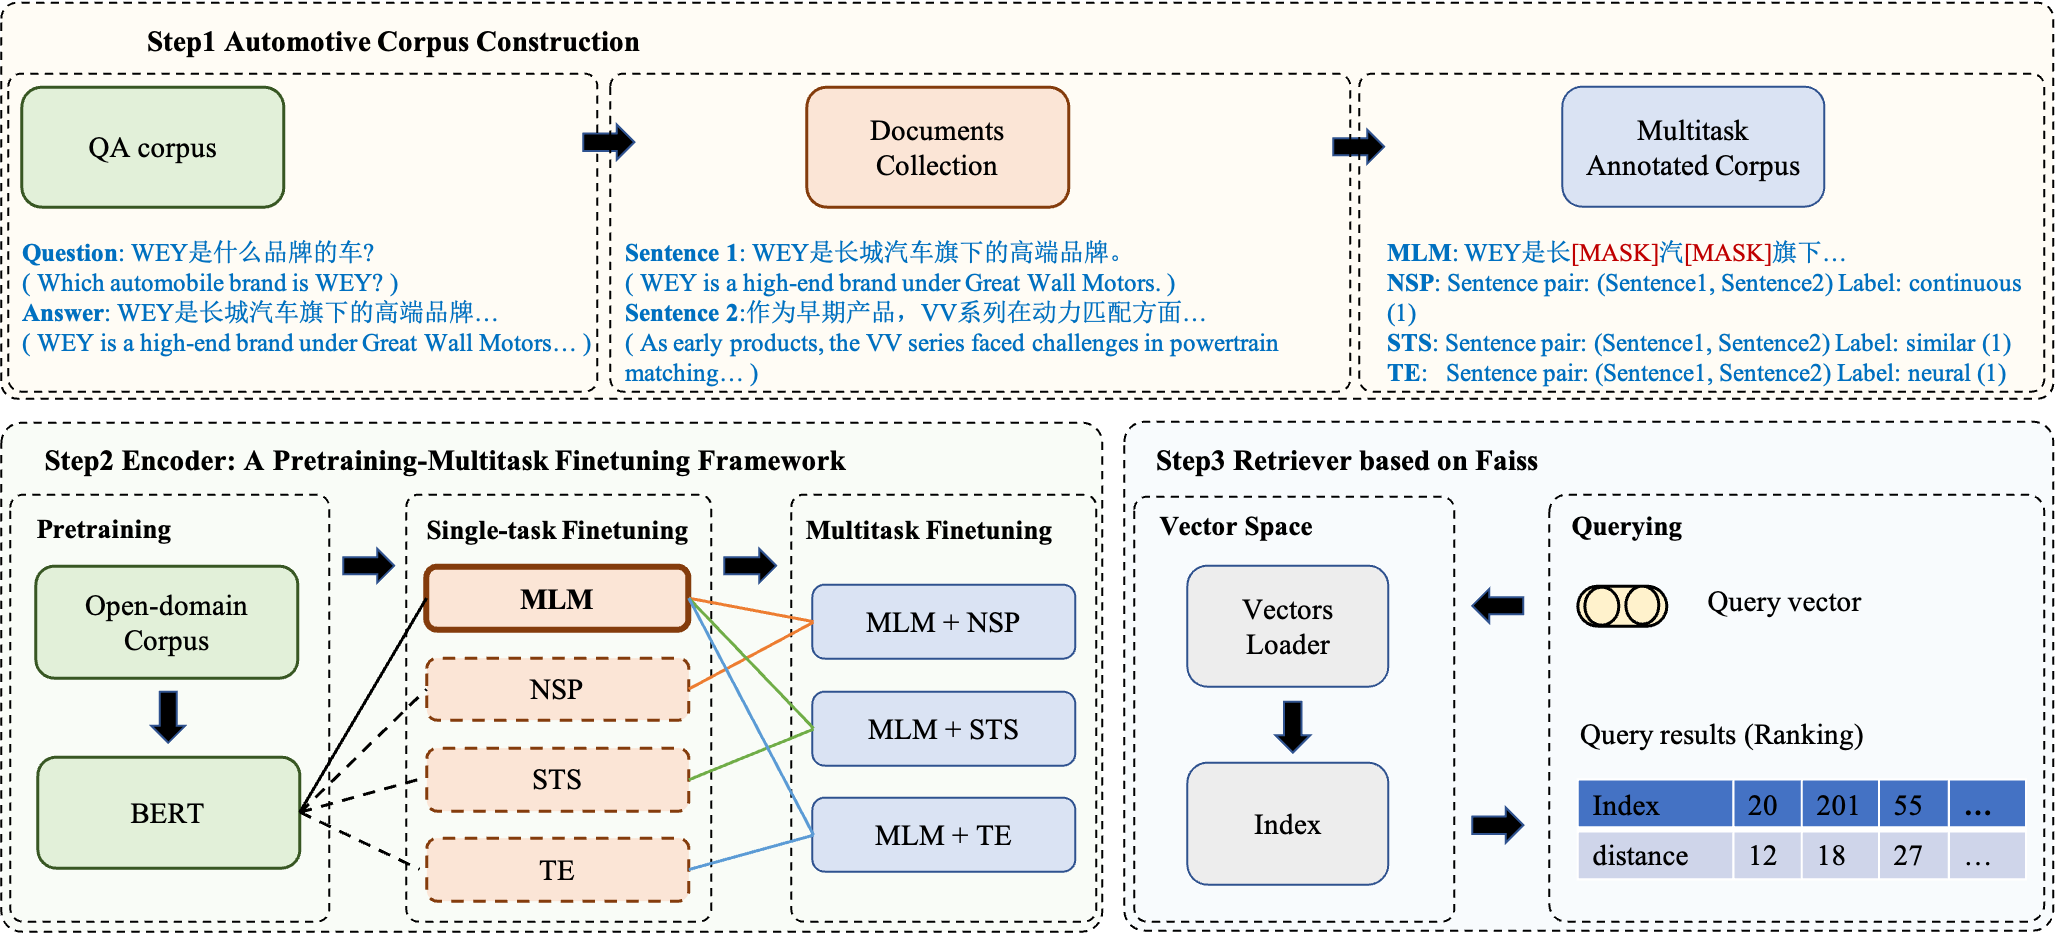
\includegraphics[width=14.0cm]{overview}
	\caption{An overview of our retrieval-based QA system. \textbf{(a) Step 1}: Automotive Corpus Construction. \textbf{(b) Step 2}: The encoder module under a pretraining-multitask fine-tuning framework. \textbf{(c) Step 3}: The retriever module based on Faiss library.}
	\label{fig:overview}
\end{figure}   
\unskip

\subsection{Corpus Construction}
\label{sec:corpus_construction}
We construct a QA dataset specific to the automotive domain by gathering question-answer pairs from authoritative resources, including professional databases, websites and other relevant resources. This dataset comprises a total of 7,157 question-answer pairs, with each pair consisting of a question and its corresponding answer. \tableref{tab:base_corpus} provides an illustrative example of the dataset. 

\begin{table}[H] 
	\caption{The constructed Chinese QA corpus in automotive domain.} \label{tab:base_corpus}
	\newcolumntype{C}{>{\centering\arraybackslash}X}
	\begin{tabularx}{\textwidth}{C}
		\toprule
		\textbf{An Example of QA pairs}	\\
		\midrule
		\{ ``id'': 0,~~~~~~~~~~~~~~~~~~~~~~~~~~~~~~~~~~~~~~~~~~~~~~~~~~~~~~~~~~~~~~~~ \\
		``question'': ``WEY是什么品牌的车?'',~~~~~~~~~~~~~~~~~~~~~~ \\
		~~~~~~~~~~ ({\color{blue} Which automobile brand is WEY?}) \\ 
		``answer'': ``WEY是长城汽车旗下的高端品牌…'', ~~~~~~~\\
		 ~~~~~~~~~~~~~~~~~~~~~~~~~~~~~~~~~~({\color{blue} WEY is a high-end brand under Great Wall Motors…}) \\
		\}~~~~~~~~~~~~~~~~~~~~~~~~~~~~~~~~~~~~~~~~~~~~~~~~~~~~~~~~~~~~~~~~~~~~~~~~~\\
%		\midrule
%		Entry 1		\\
%		Entry 2	Dat \textsuperscript{1}\\
		\bottomrule
	\end{tabularx}
%	\noindent{\footnotesize{\textsuperscript{1} Tables may have a footer.}}
\end{table}

Furthermore, each answer within the QA dataset is treated as an individual document, contributing to a comprehensive collection of documents focused on the automotive domain. This collection encompasses over 240K sentences, covering a wide range of automotive knowledge. It serves as the foundational resource (base corpus) for constructing multitask annotated corpus in this paper.
Backed by this base corpus, we build a multitask annotated corpus involving several tasks, including Mask Language Modeling (MLM), Next Sentence Prediction (NSP), Semantic Textual Similarity (STS), and Textual Entailment (TE). Specific examples for each task-oriented corpus are shown in Table 2.
The construction process of each task-oriented corpus is outlined as follows:
\begin{itemize}
	\item	MLM Corpus: A subset of sentences is selected from the base corpus, and a certain proportion of words are randomly masked. The MLM corpus is created by annotating the original words in the masked positions.
	\item	NSP Corpus: Each example consists of two sentences. A certain proportion of sentence pairs are randomly selected from the base corpus. Half of the pairs consist of consecutive sentences, labeled as 1, while the other half consist of randomly selected sentence pairs, labeled as 0.
	\item STS Corpus: The STS corpus is constructed by paraphrasing sentences from the base corpus. To ensure a balanced corpus, positive and negative examples are generated in equal proportions. 50\% of the sentences from the document collection are randomly sampled and paraphrase into similar sentences using iFlytek tools. The paraphrased sentences are then filtered by annotators, and those deemed similar to the original sentences are selected as positive examples (labeled as 1, similar). Negative examples are generated by employing a random matching method, where sentences of similar length to the positive examples are randomly sampled and pair to form negative examples (labeled as 0, dissimilar). This approach maintains consistency in length between positive and negative examples, thereby facilitating model training.
	\item	TE Corpus: To construct the TE corpus, we extracted 880,000 annotated examples from an existing Chinese Textual Entailment dataset. Each example includes a premise and a hypothesis. Based on the inference relationship between the two, they were labeled as entailment (0), contradiction (2), or neutral (1).
\end{itemize}

\begin{table}[H] 
	\caption{The constructed Chinese QA corpus in automotive domain.} \label{tab:annotated_corpus}
	\newcolumntype{C}{>{\centering\arraybackslash}X}
	\begin{tabularx}{\textwidth}{p{2cm}L} 
		\toprule
		\textbf{Name}  & \textbf{Data Format}	\\
		\midrule
		MLM Corpus  & \textbf{[MASK][MASK]}车队首次在1994年的JGTC第四站比\textbf{[MASK]}中亮相,获得了资格赛第二名的位置。{\color{blue} (The [MASK] team made its debut in the fourth round of the JGTC  in 1994, securing the second position in the qualifying [MASK].) } \\
		\midrule
		NSP Corpus  & \textbf{Sentence1}: 上世纪90年代,TRD为丰田TOM'S车队打造了Supra赛车。{\color{blue} (In the 1990s, TRD built Supra race cars for the Toyota TOM'S team.) }
		\textbf{Sentence2}: 丰田车队首次在1994年的JGTC第四站比赛中亮相,获得了资格赛第二名的位置。{\color{blue} (The Toyota team made its debut in the fourth round of the JGTC  in 1994, securing the second position in the qualifying race.)} ~~~~~~~~~~~~~~~~~~~~~~~~~~~~~~~~\textbf{Label}: continuous (1)\\
		\midrule
		STS Corpus & \textbf{Sentence1}: 丰田车队首次在1994年的JGTC第四站比赛中亮相,获得了资格赛第二名的位置。{\color{blue} (The Toyota team made its debut in the fourth round of the JGTC  in 1994, securing the second position in the qualifying race.)}
		\textbf{Sentence2}: 在1994年的JGTC第四站比赛中,丰田车队首次参赛,并在资格赛中获得了第二名的成绩。{\color{blue} (In 1994, during the fourth round of the JGTC, the Toyota team made its debut and secured a second-place finish in the qualifying race.)} ~~~~~~~~~~~~~~~~~~~~~~~~~~~~~~~~~~~~~~~~~~~~~~~~~~~~~~~~~~~~~~~~~~~~~~~~~ \textbf{Label}: similar (1) ~~~~~~~~		\\
		\midrule
		TE Corpus  &  \textbf{Sentence1}: 一个年轻的黑人正试图向另外两个人解释一些事情。{\color{blue} (A young black person is trying to explain something to two other individuals.)}
		\textbf{Sentence2}: 一位年轻的黑人男子正在和另外两位说话。{\color{blue} (A young black man is talking to two other people.)} ~~~~~~~~~~~~~~~~~~~~~~~~~~~~~~~~~~~~~~~~~~~~~~~~~~~~~~~~~~~~~ \textbf{Label}: entailment (0) ~~~~~		\\
		\bottomrule
	\end{tabularx}
	%	\noindent{\footnotesize{\textsuperscript{1} Tables may have a footer.}}
\end{table}

\subsection{Encoder: A Pretraining-Multitask Fine-tuning Framework}
\label{sec:encoder}


Based on the multitask corpus constructed in \secref{sec:corpus_construction}, we propose a joint learning framework with a pretraining-multitask fine-tuning architecture. The objective of this framework is to integrate auxiliary task objectives and develop a specialized encoder specifically designed for the automotive domain. By incorporating domain knowledge, our framework enables better adaptation to downstream task requirements in the automotive domain.

To be more  specific, we propose a multitask fine-tuning strategy based on the pretrained BERT model, as illustrated in \figref{fig:overview} (b). Firstly, we individually fine-tune the pretrained model  on the MLM, NSP, TE, and STS tasks. Then, we evaluate the impact of each task on the model's performance through comparative analysis.  Based on this evaluation, we identify the fine-tuning tasks that have a positive influence on the model and designate them as the main tasks. In the subsequent stage of multitask fine-tuning, we engage in joint learning, where the main task is learned alongside other auxiliary tasks. This strategy fosters mutual reinforcement and interactive learning among tasks by selecting auxiliary tasks that interact positively with the main task, sharing parameters, and training collaboratively. Through this joint learning approach, the model is able to fully leverage the correlations and complementarities among different tasks, leading to further improvements in its performance on specific domain tasks.

Regarding the specific parameter settings during the fine-tuning stage for each task, the following configurations are applied: a batch size of 16, a dropout rate of 0.1 for attention layers, a dropout rate of 0.1 for hidden layers, 768 hidden units, a learning rate of 5e-5, linear decay as the gradient decay strategy, utilization of the BERTAdam optimizer with weight decay of 0.01, and a training duration of 3 epochs. For the MLM fine-tuning, a masking rate of 15\% is applied. The maximum sequence length is set to 512 for all tasks, except for TE, as the TE corpus contains shorter sentence pairs. Consequently, the maximum sequence length during fine-tuning for TE is set to 256.

%Numbered lists can be added as follows:
%\begin{enumerate}
%\item	First item; 
%\item	Second item;
%\item	Third item.
%\end{enumerate}
%
%The text continues here. 

\subsection{Retriever based on Faiss}
\label{sec:retriever}
Faiss (Facebook AI Similarity Search) is \DIFdelbegin \DIFdel{an }\DIFdelend \DIFaddbegin \DIFadd{a highly }\DIFaddend efficient open-source library \DIFaddbegin \DIFadd{designed specifically }\DIFaddend for vector retrieval\DIFdelbegin \DIFdel{, offering }\DIFdelend \DIFaddbegin \DIFadd{. It provides robust }\DIFaddend support for various vector index structures and similarity calculation methods. \DIFdelbegin \DIFdel{. It excels at efficiently handling }\DIFdelend \DIFaddbegin \DIFadd{One of its notable strengths lies in its efficient handling of }\DIFaddend large-scale vectors, \DIFdelbegin \DIFdel{making it well-suited }\DIFdelend \DIFaddbegin \DIFadd{rendering it highly suitable }\DIFaddend for industrial-grade applications. \DIFdelbegin \DIFdel{To }\DIFdelend \DIFaddbegin \DIFadd{In our efforts to }\DIFaddend further enhance the retrieval efficiency of the system, we \DIFdelbegin \DIFdel{introduce a }\DIFdelend \DIFaddbegin \DIFadd{have introduced a dedicated }\DIFaddend vector retrieval module that \DIFdelbegin \DIFdel{leverages the Faiss framework.
}\DIFdelend \DIFaddbegin \DIFadd{harnesses the power of the Faiss framework, as depicted in \figref{fig:overview} (c).
%DIF > To further enhance the retrieval efficiency of the system, we introduce a vector retrieval module that leverages the Faiss framework, as illustrated in \figref{fig:overview} (c). 
We first construct the vector space by loading the base corpus as supporting vectors using encoder illustrated in \figref{fig:overview} (b). These vectors are then indexed using the IndexFlat2 structure, which is based on the Faiss library. Upon receiving a query, the retriever module first converts it into a query vector and then performs a search within the vector space to identify the most similar targets. Subsequently, a ranking is generated, presenting the top K matching questions along with their corresponding answers.
%DIF > Initially, we construct the vector space by loading base corpus as supporting vectors. These vectors are indexed using the IndexFlat2 structure based on the Faiss library. When a query is received by our system, it is first converted into a query vector, and then a search is performed within the vector space to find the most similar targets.
%DIF > Finally, a ranking is generated, which includes the top K matching questions along with their corresponding answers. 
}\DIFaddend 


When constructing the IndexFlatL2 index, the L2 norm of each vector in the vector dataset is computed and stored in the index file along with its corresponding vector. This enables fast computation of the L2 distance between the query vector and the stored vectors during the query phase. 
Assuming the query vector is denoted as $\mathbf{x}$ and any stored vector as $\mathbf{y}$, \eqnref{eq:l2} describes the computation of the squared L2 distance between $\mathbf{x}$ and $\mathbf{y}$:
\begin{linenomath}
	\begin{equation}\label{eq:l2}
		||\mathbf{x}-\mathbf{y}||_2^2 = ||\mathbf{x}||_2^2 + ||\mathbf{y}||_2^2 - 2\mathbf{x}\cdot \mathbf{y}, 
	\end{equation}
\end{linenomath}
where $\mathbf{y}||_2^2$ represents the square of the L2 norm of the stored vector, which is precomputed and stored in the index.

During the query phase, the precomputed L2 norms are utilized to calculate the distance, eliminating the need for redundant computations. After constructing the index, the vector set is organized into a retrieval vector space. In the querying process, the vector representation of the query text is introduced into the index as the target, and a search is performed in the retrieval space to compute the L2 distance between the query vector and the stored vectors. By leveraging the IndexFlatL2 index, the retrieval system efficiently computes the L2 distance between the query vector and the stored vectors, enabling similarity ranking and nearest neighbor search based on the distance. The system returns the top K most similar vector indices and subsequently extracts the corresponding question text and relevant information based on these indices.
%\begin{equation}\label{eq:tag_loss}
%	L_{tag}=-\sum_{x\in D}\sum_{i=1}^{L(x)} \log (p(t_i | x_{i})) ,
%\end{equation}
%The proposed retriever utilizes the IndexFlat2 for efficient storage and retrieval vectors. 

\section{Experiments}
In this section, we first create an evaluation dataset for the automotive domain. Next, we introduce evaluation metrics utilized in our experiments. Finally, we conduct a comparative analysis against competing models to substantiate the effectiveness of our system.

\subsection{Evaluation Dataset}
Firstly, we create a retrieval corpus (shown in \tableref{tab:question_set}) utilizing the question set outlined  in \secref{sec:corpus_construction}. 
Then, we randomly sample 100 questions from the retrieval corpus. These selected questions are then subjected to synonymous rephrasing using ChatGPT, which ultimately leads to the creation of the evaluation dataset (shown in \tableref{tab:eval_dataset}).

\begin{table}[H] 
	\caption{The retrieval corpus consisted of all questions in QA dataset.} \label{tab:question_set}
	\newcolumntype{C}{>{\centering\arraybackslash}X}
	\begin{tabularx}{\textwidth}{C}
		\toprule
		\textbf{Questions}	\\
		\midrule
		\{ 未来车门会是什么样?\} \\({\color{blue} What will the car doors of the future look like?})\\
		\midrule
		\{ WEY是什么品牌的车?\} \\({\color{blue} Which automobile brand is WEY?}) \\ \midrule
		\{ 长安沃尔沃和吉利沃尔沃有什么区别?\} \\ ({\color{blue} What is the difference between Changan Volvo and Geely Volvo?})\\
		%		\midrule
		%		Entry 1		\\
		%		Entry 2	Dat \textsuperscript{1}\\
		\bottomrule
	\end{tabularx}
	%	\noindent{\footnotesize{\textsuperscript{1} Tables may have a footer.}}
\end{table}

Specifically, we transform the rephrasing task description and the question text into prompts, which are fed into ChatGPT to generate the rephrased results. These results are then subject to manual screening to create the final evaluation dataset. The prompts are designed following specific principles: (1) Role assignment: ChatGPT assumes the role of an automotive engineer, for instance, with a prompt like ``Imagine you are an automotive engineer''. (2) Rephrasing task description: a detailed explanation of the rephrasing task requirements is provided, such as ``You will receive a text related to the automotive domain and your task is to rewrite it, ensuring that the length remains similar to the original while preserving its meaning''. (3) Result requirements: the desired outcomes of ChatGPT's generation are described, for example, with a prompt like ``Please provide 6 rephrased results for each data point and rank them in descending order based on their quality''. Subsequently, human annotators manually review the rephrased results generated by ChatGPT, carefully examining each question's rephrased versions, and selecting the top 4 synonyms with the highest quality. This process yields a dataset comprising 400 user queries, as depicted in Table 4. Each query corresponds to a question in the {\em queries} field and has a corresponding reference question in the retrieval corpus, indicated by the {\em reference} field. This user query dataset is utilized to evaluate the performance of the retrieval-based question answering model.

\begin{table}[H] 
	\caption{The evaluation dataset in our experiments.} \label{tab:eval_dataset}
	\newcolumntype{C}{>{\centering\arraybackslash}X}
	\begin{tabularx}{\textwidth}{L}
	\toprule
		\textbf{An illustration Example}	\\
		\midrule
		\{ ``reference'': ``长安cs75plus车型热销背后的几点思考'',~~~~~~~~~~~~~~~~~~~~~~~~~~~~~~~ \\
		~~~~~~~~~~~~~~~~~~~({\color{blue} Some thoughts behind the hot sales of the Changan CS75 Plus model.}) \\ 
		~~~``queries'': [\\
		~~~~~~``长安cs75plus车型热销背后原因解析'', \\
		~~~~~~~({\color{blue} Analysis of the reasons behind the high sales of the Changan CS75 Plus model.}) \\ 
		~~~~~~``购买长安cs75plus车型的几点原因'', \\
		~~~~~~ ({\color{blue} Several reasons for purchasing the Changan CS75 Plus model.}) \\ 
		~~~~~~``长安cs75plus车型为什么能够热销,列出几点原因'', \\
		~~~~~~~({\color{blue} Please list a few reasons to explain why the Changan CS75 Plus model sells well.}) \\ 
		~~~~~~~``长安cs75plus车型,热销背后的原因思考'',~~~~ \\
		~~~~~~ ({\color{blue} Reflection on the reasons behind the popularity of the Changan CS75 Plus model.}) \\ 
		~~~~] ~~~~~~~~~~~~~~~~~~~~~~~~~~~\\
		\}~~~~~~~~~~~~~~~~~~~~~~~~~~~~~~~~~~~~~~~~~~~~~~~~~~~~~~~~~~~~~~~~~~~~~~~~~\\
		\bottomrule
	\end{tabularx}
	%	\noindent{\footnotesize{\textsuperscript{1} Tables may have a footer.}}
\end{table}


\subsection{Evaluation Metrics}
\label{sec:metrics}
The hit rate at K (Hit@K) is a widely used evaluation metric for assessing the performance of retrieval systems. It measures the capability to rank the correct target of user queries among the top K retrieval results. When conducting Hit@K for evaluation, a query is considered a hit if the true target is included in the top K retrieval results; otherwise, it is categorized as a miss. In our experiments, we utilize Hit@1, Hit@3, and Hit@5 as evaluation metrics for the retrieval model. Formally, the Hit@K is computed as:
\begin{linenomath}
	\begin{equation}\label{eq:hit}
		Hit@K = \frac{N_K}{|\mathcal{Q}|}, 
	\end{equation}
\end{linenomath}
where $N_K$ represents the total number of hits for $N$ retrieval tasks, and $|\mathcal{Q}|$ is the total number of true targets across all queries.

While Hit@K is a straightforward metric, it solely focuses on the top-ranked results, disregarding other potentially valuable outcomes. To account for the ranking of all results, we utilize the Mean Reciprocal Rank (MRR) as an evaluation metric. MRR is computed as follows:
\begin{linenomath}
	\begin{equation}\label{eq:mrr}
		MRR = \frac{1}{|S|}\sum_{i=1}^{|S|}\frac{1}{r_i}, 
	\end{equation}
\end{linenomath}
where $|S|$ represents the total number of queries, and $r_i$ denotes the ranking of the true target corresponding to the $i$-th query in the retrieved  results.

In addition, we present a novel evaluation metric designed based on real user behavior. Considering that the result page of the QA system  has the capability to display multiple results, the difference between the top-ranked and fifth-ranked feedback results holds minimal significance in terms of user experience. However, the MRR metric assigns a score difference of 0.8 between the first and fifth ranks (with a maximum score of 1). 
Moreover, considering that users typically limit their exploration to the initial pages of retrieval results, if a rank exceeds a certain threshold, it indicates a failure of the query sample to produce the correct result within the system. Despite a low ranking, MRR still provides a positive evaluation score when used for assessment. To address these concerns, we propose a new evaluation metric called Mean Linear Window Rank (MLWR). MLWR linearly adjusts the impact of ranking on the evaluation metric and incorporates a window size to exclude query samples with rankings beyond the predefined window. This approach better aligns with the user experience requirements of the system and provides a comprehensive assessment of retrieval system performance. Formally, MLWR is computed as follows:
\begin{linenomath}
	\begin{equation}\label{eq:mlwr}
		MLWR = \sum_{i=1}^{|S|}\frac{\max\{0, N-r_i+1\}}{N\times |S|}, 
	\end{equation}
\end{linenomath}
where $|S|$ represents the total number of samples, $r_i$ denotes the ranking of the true target corresponding to the $i$-th query in the retrieved  results, and $N$ is the window size. 

\subsection{Comparison Results}
In this section, we compare the performance of pretrained models, single-task fine-tuned models, and multitask fine-tuned models on the automotive domain QA retrieval task. By thoroughly examining the experimental results, we identify the most effective multitask fine-tuning strategy.

Based on the multitask annotated corpus (see \secref{sec:corpus_construction}) and the single-task fine-tuning strategy (see \secref{sec:encoder}), we perform individual fine-tuning on the general pre-trained model for the MLM, TE, NSP, and STS tasks. This process yields four fine-tuned models: FT-MLM model (fine-tuned with BERT model for the MLM task), FT-TE model (fine-tuned with BERT model for the TE task), FT-NSP model (fine-tuned with BERT model for the NSP task), and FT-STS model (fine-tuned with \DIFdelbegin \DIFdel{BERT }\DIFdelend \DIFaddbegin \DIFadd{pre-trained }\DIFaddend model for the STS task). Subsequently, we compare and analyze the performance of these four fine-tuned models alongside the baseline \DIFdelbegin \DIFdel{BERT }\DIFdelend \DIFaddbegin \DIFadd{$\text{BERT}_{base}$ }\DIFaddend model using the evaluation metrics introduced in \secref{sec:metrics}. The experimental results, presented in \tableref{tab:single}, reveal that two text encoding methods, namely CLS and MEAN, are employed in the experiments. CLS encoding extracts the [CLS] vector from the final layer of the model encoder as the encoded output of the text, while MEAN encoding performs average pooling on the outputs of each token in the final layer of the model encoder, producing an averaged pooling vector as the encoded output. Both of these encoding methods are utilized in the construction of the fine-tuned models and are compared in our experiments.

\begin{table}[H] 
	\caption{Comparison of Hit@K, MRR, MLWR using single-task fine-tuning models \DIFaddbeginFL \DIFaddFL{based on $\text{BERT}_{base}$}\DIFaddendFL .} \label{tab:single}
	\newcolumntype{C}{>{\centering\arraybackslash}X}
	\begin{tabularx}{\textwidth}{p{1.5cm}CCCCCCCCCC}
		\toprule
		\multirow{2}{*}{\textbf{Model}} & \multicolumn{2}{c}{Hit@1(\%)} & \multicolumn{2}{c}{Hit@3(\%)} & \multicolumn{2}{c}{Hit@5(\%)} & \multicolumn{2}{c}{MRR(\%)} & \multicolumn{2}{c}{MLWR(\%)} \\
		\cline{2-11} 
		\addlinespace
		& CLS           & MEAN          & CLS           & MEAN          & CLS           & MEAN          & CLS          & MEAN         & CLS           & MEAN         \\
		\midrule
		\DIFdelbeginFL \DIFdelFL{BERT   }\DIFdelendFL \DIFaddbeginFL \DIFaddFL{$\text{BERT}_{base}$   }\DIFaddendFL & 30.00         & 64.50         & 39.50         & 72.25         & 43.25         & 77.25         & 36.57        & 70.21        & 47.37         & 79.97   \\ 
%DIF > 		BERT   & 30.00         & 64.50         & 39.50         & 72.25         & 43.25         & 77.25         & 36.57        & 70.21        & 47.37         & 79.97        \\
		FT-MLM & 47.25         & 77.00         & 55.50         & 83.50         & 57.00         & 85.75         & 52.19        & 80.94        & 58.96         & 86.76        \\
		FT-STS & 13.00         & 60.25         & 18.50         & 71.25         & 22.25         & 74.75         & 17.73        & 66.58        & 26.21         & 76.19        \\
		FT-TE  & 5.00          & 24.75         & 8.50          & 30.25         & 9.00          & 32.75         & 7.27         & 28.89        & 10.73         & 35.41        \\
		FT-NSP & 14.75         & 59.00         & 14.75         & 67.75         & 20.75         & 71.00         & 18.53        & 64.53        & 24.56         & 73.29  \\ 
%DIF > 		$\text{BERT}_{large}$   & 26.50         & 64.50         & 39.50         & 72.25         & 43.25         & 77.25         & 36.57        & 70.21        & 47.37         & 79.97   \\ 
		\bottomrule
	\end{tabularx}
	%	\noindent{\footnotesize{\textsuperscript{1} Tables may have a footer.}}
\end{table}


As shown in \tableref{tab:single}, the general baseline BERT model exhibits poor performance in the automotive domain retrieval question-answering task. The Hit@1, using CLS encoding, is a mere 30\%, with an MLWR of 47.37\%. Conversely, the Hit@1, employing MEAN encoding, reaches 64.5\%, accompanied by an MLWR of 79.97\%. This highlights the improvement achieved by applying average pooling to the encoder outputs in enhancing representations for domain-specific texts. Individually fine-tuning the BERT model with the MLM task, based on the domain-specific corpus, yields a significant performance boost. The FT-MLM model attains a Hit@1 of 47.25\% and 77\% under CLS encoding and MEAN encoding, respectively. These figures reflect improvements of 17.25 and 12.5 percentage points compared to the BERT model. Furthermore, the MLWR is enhanced to 58.96\% and 86.76\%, respectively, corresponding to gains of 11.59 and 6.79 percentage points over the BERT model. Thus, MLM single-task fine-tuning, grounded in the automotive domain corpus, proves highly effective in enhancing model performance. Additionally, \tableref{tab:single} shows that individual fine-tuning of the BERT model with the STS, TE, and NSP tasks results in a certain degree of performance decline. Notably, the negative impact on model performance from fine-tuning the NSP and STS tasks is relatively minor, further substantiating their potential positive contribution to model performance when engaged as auxiliary tasks in the multi-task fine-tuning framework.

The preceding analysis provides valuable guidance for the subsequent steps involved in establishing multitask fine-tuning strategies. According to \tableref{tab:single}, it is evident that selecting the MLM task as the primary task and incorporating appropriate auxiliary tasks for joint learning is an effective strategy for multitask fine-tuning. To further investigate the potential positive interactions between MLM and other auxiliary tasks within the multitask fine-tuning framework, we proceed to fine-tune the baseline model using the MLM+STS and MLM+NSP multitask learning methods. A comparative analysis is performed against the FT-MLM model to evaluate the actual contributions of the NSP and STS tasks in the context of multitask fine-tuning. The performance results of the models under multitask fine-tuning are presented in \tableref{tab:multi}.


\begin{table}[H] 
	\caption{Comparison of Hit@K, MRR, MLWR using multitask fine-tuning models \DIFaddbeginFL \DIFaddFL{based on $\text{BERT}_{base}$}\DIFaddendFL .} \label{tab:multi}
	\newcolumntype{C}{>{\centering\arraybackslash}X}
	\begin{tabularx}{\textwidth}{p{3.0cm}CCCCCC}
	\toprule
	\multicolumn{1}{c}{Model}                & Hit@1(\%) & Hit@3(\%) & Hit@5(\%) & MRR(\%) & MLWR(\%) \\
	\midrule
	STS+MLM {[}CLS{]}  & 74.25     & 84.00     & 85.25     & 79.54   & 87.12    \\
	NSP+MLM {[}CLS{]}  & 8.25      & 15.00     & 18.75     & 13.08   & 21.65    \\
	STS+MLM {[}MEAN{]} & 77.50     & 84.75     & 87.00     & 81.60   & 87.71    \\
	NSP+MLM {[}MEAN{]} & 73.25     & 78.75     & 80.50     & 76.77   & 82.17   \\
	\bottomrule
	\end{tabularx}
	%	\noindent{\footnotesize{\textsuperscript{1} Tables may have a footer.}}
\end{table}


As shown in \tableref{tab:single} and \tableref{tab:multi}, the performance of the multitask fine-tuning models (NSP+MLM and STS+MLM) is significantly better than that of the baseline BERT model, further validating the effectiveness of fine-tuning the models based on domain-specific task corpora. From \tableref{tab:multi}, it is evident that under MEAN encoding, the performance of the STS/NSP task+MLM multi-task fine-tuning models consistently outperforms that of the STS/NSP single-task fine-tuning models, which again demonstrates the rationale for selecting the MLM task as the main task during the multi-task fine-tuning phase. However, the NSP+MLM fine-tuning model performs slightly worse than the single-task FT-MLM model (see \tableref{tab:multi}), and even under single-task fine-tuning, the performance of the FT-NSP model is still slightly inferior to that of the baseline BERT model (see \tableref{tab:single}). This indicates that involving the NSP task in fine-tuning is not beneficial for downstream retrieval-based question-answering applications. Previous works, such as RoBERTa~\cite{roberta} and SpanBERT~\cite{spanbert}, have also found that using the NSP task as a pretraining objective leads to a performance decline when handling question-answering tasks. This could be due to the fact that the NSP task aims to determine whether two sentences are consecutive, which is not directly related to the objective of question-answering tasks, and the joint learning of NSP and MLM tasks fails to generate positive effects. For the STS task, under both CLS and MEAN encoding, the performance of the STS+MLM joint fine-tuning model consistently outperforms that of the single-task MLM fine-tuning model, with Hit@1 reaching 74.25\% and 77.5\% respectively, which represents improvements of 27 and 0.5 percentage points compared to the FT-MLM model. The MLWR reaches 87.12\% and 87.71\% respectively, with improvements of 28.16 and 0.95 percentage points compared to the FT-MLM model.



\DIFdelbegin \DIFdel{Based on the performance comparisons of the models in \tableref{tab:single} and \tableref{tab:multi}, it can be concluded that : 1) The performance of the models based on MEAN encoding is significantly better than that based on CLS encoding; 2)Using MLM single-task, }\DIFdelend \DIFaddbegin \begin{table}[H] 
	\caption{\DIFaddFL{Comparison of Hit@K, MRR, MLWR using the best single-task and multitask fine-tuning models based on $\text{BERT}_{large}$ and $\text{RoBERTa}$.}} \label{tab:sup}
	\newcolumntype{C}{>{\centering\arraybackslash}X}
	\begin{tabularx}{\textwidth}{p{1.5cm}CCCCCCCCCC}
		\toprule
		\multirow{2}{*}{\textbf{Model}} & \multicolumn{2}{c}{Hit@1(\%)} & \multicolumn{2}{c}{Hit@3(\%)} & \multicolumn{2}{c}{Hit@5(\%)} & \multicolumn{2}{c}{MRR(\%)} & \multicolumn{2}{c}{MLWR(\%)} \\
		\cline{2-11} 
		\addlinespace
		& \DIFaddFL{CLS           }& \DIFaddFL{MEAN          }& \DIFaddFL{CLS           }& \DIFaddFL{MEAN          }& \DIFaddFL{CLS           }& \DIFaddFL{MEAN          }& \DIFaddFL{CLS          }& \DIFaddFL{MEAN         }& \DIFaddFL{CLS           }& \DIFaddFL{MEAN         }\\
		\toprule
		\DIFaddFL{$\text{BERT}_{large}$   }& \DIFaddFL{26.50         }& \DIFaddFL{64.50         }& \DIFaddFL{39.50         }& \DIFaddFL{72.25         }& \DIFaddFL{43.25         }& \DIFaddFL{77.25         }& \DIFaddFL{36.57        }& \DIFaddFL{70.21        }& \DIFaddFL{47.37         }& \DIFaddFL{79.97   }\\ 
		\DIFaddFL{FT-MLM }& \DIFaddFL{29.25         }& \DIFaddFL{76.75         }& \DIFaddFL{36.50         }& \DIFaddFL{82.00         }& \DIFaddFL{39.50         }& \DIFaddFL{85.25        }& \DIFaddFL{33.88        }& \DIFaddFL{80.42        }& \DIFaddFL{41.56        }& \DIFaddFL{86.19        }\\
		\DIFaddFL{MLM+}\DIFaddendFL STS \DIFdelbeginFL \DIFdelFL{single-task, and }\DIFdelendFL \DIFaddbeginFL & \DIFaddFL{18.50        }& \DIFaddFL{78.00        }& \DIFaddFL{22.20         }& \DIFaddFL{83.50        }& \DIFaddFL{23.50         }& \DIFaddFL{85.75         }& \DIFaddFL{21.13       }& \DIFaddFL{81.67     }& \DIFaddFL{25.16       }& \DIFaddFL{88.42      }\\ \toprule[0.2mm]
		\DIFaddFL{$\text{RoBERTa}$   }& \DIFaddFL{69.00         }& \DIFaddFL{73.00         }& \DIFaddFL{77.75      }& \DIFaddFL{79.50        }& \DIFaddFL{79.25        }& \DIFaddFL{82.75        }& \DIFaddFL{74.16        }& \DIFaddFL{77.41       }& \DIFaddFL{81.59         }& \DIFaddFL{84.61   }\\ 
		\DIFaddFL{FT-MLM }& \DIFaddFL{73.25        }& \DIFaddFL{75.75        }& \DIFaddFL{79.25        }& \DIFaddFL{81.75        }& \DIFaddFL{83.25         }& \DIFaddFL{84.00         }&  \DIFaddFL{77.63        }& \DIFaddFL{79.79        }& \DIFaddFL{85.31         }& \DIFaddFL{86.81        }\\
		\DIFaddendFL MLM\DIFdelbeginFL \DIFdelFL{+STSmultitask as }\DIFdelendFL \DIFaddbeginFL \DIFaddFL{+STS }& \DIFaddFL{37.50         }& \DIFaddFL{78.75        }& \DIFaddFL{48.25         }& \DIFaddFL{84.50       }& \DIFaddFL{51.75        }& \DIFaddFL{87.75         }& \DIFaddFL{44.46     }& \DIFaddFL{82.50       }& \DIFaddFL{55.16         }& \DIFaddFL{88.79       }\\
		\bottomrule[0.2mm]
	\end{tabularx}
	%DIF > 	\noindent{\footnotesize{\textsuperscript{1} Tables may have a footer.}}
\end{table}


\DIFadd{To illustrate the generalization capability of our framework in mitigating bias within pretrained models, we extend our evaluation beyond the BERT-base model to also include the BERT-large and RoBERTa models. As shown in \tableref{tab:sup}, our framework exhibits effective generalization   across a variety of pretrained models. It is worth nothing that RoBERTa, which is solely pretrained using the MLM task, demonstrates good performance with the CLS encoding, achieving a Hit@1 score of 69\%. However, in pretraining models such as BERT-base and BERT-large, the CLS representation primarily learns from the NSP task, resulting in sub-optimal performance when directly utilizing the  CLS encoding. These findings highlight the negative impact of the NSP task as a training objective on QA tasks, while emphasizing the benefits of the MLM task as a training objective for downstream QA tasks. 
}

%DIF > Furthermore, in order to showcase the effectiveness of the retriever module in our proposed system, we compare its performance using different indexing structures as described in Section 3.2. Specifically, we evaluate the retriever module using brute force, IndexPQ index, IndexHNSWFlat, and IndexFlatL2. 
%DIF > As shown in 
\subsection{\DIFadd{Case Study}}
\DIFadd{In this section,  we conduct a case study to qualitatively analyze competing models. 
\tableref{tab:case} presents the results obtained when inputting an example user query, 
namely ``如何对高尔夫7系列车型进行自我检修?'' (}{\color{blue} \DIFadd{How to perform self-maintenance on Volkswagen Golf7 series?}}\DIFadd{), and showcases the responses retrieved by the competing models utilizing $\text{BERT}_{base}$ in proposed framework.
The baseline BERT model provides a historical overview of the 7th Generation Volkswagen Golf, while the single-task FT-MLM model compares the 308S and Golf 7 models. However, neither of these models is capable of providing an accurate answer to the query. In contrast, the STS+MLM joint }\DIFaddend fine-tuning \DIFdelbegin \DIFdel{objectives can enhance the performance of the language model in downstream automotive domain retrieval-based question-answering tasks}\DIFdelend \DIFaddbegin \DIFadd{model effectively responds with the precise and specific steps to perform maintenance on the FAW-Volkswagen Golf7, thereby correctly addressing the query.
The STS+MLM joint model demonstrates its effectiveness in capturing the query intentions, surpassing other competing models in terms of qualitative performance}\DIFaddend .


\DIFaddbegin \begin{table}[H] 
	\caption{\DIFaddFL{Retrieved answers from baseline $\text{BERT}_{base}$ model, single-task FT-MLM model, and multitask STS+MLM model.}} \label{tab:case}
	\newcolumntype{C}{>{\centering\arraybackslash}X}
	\begin{tabularx}{\textwidth}{cp{10cm}}
		\toprule
		\multicolumn{2}{p{12cm}}{\hangindent=2.2cm \hangafter=1 \textbf{Input Query}: ``如何对高尔夫7系列车型进行自我检修?'' ({\color{blue} How to perform self-maintenance on Volkswagen Golf7 series?})}   \\
		\midrule
		\textbf{\DIFaddFL{Model}} & \textbf{\DIFaddFL{Retrieved answers}} \\ \midrule
		\DIFaddFL{$\text{BERT}_{base}$  }&  \DIFaddFL{1. 高尔夫Mk1:1974年5月,第一代高尔夫... 2. 高尔夫Mk2:1983年8月,大众推出第二代... (}{\color{blue} \DIFaddFL{1. Golf Mk1: In May 1974, the first generation Golf was introduced..  2. Golf Mk2: In August 1983, Volkswagen unveiled the second generation...}}\DIFaddFL{)  }\\\midrule
		\DIFaddFL{FT-MTM  }&       \DIFaddFL{1. 动力组合对比:高尔夫一共有三种排量...	 2. 质保政策对比:高尔夫官方保修周期为3年或者...
		  (}{\color{blue} \DIFaddFL{1. Powertrain Comparison: The Golf is available in three different engine displacements... 2. Warranty Policy Comparison: The official warranty period for the Golf is 3 years or...}}\DIFaddFL{)   }\\ \midrule
		\DIFaddFL{MLM+STS  }&   \DIFaddFL{1. 更换4.5升5w40美孚全合成机油、博世机滤、博世空气滤芯、博世空调滤芯、博世汽油滤芯、3m燃油添加剂、免拆三元催化清洗剂
2. 动平衡、更换原厂轮毂盖
		 (}{\color{blue} \DIFaddFL{1. Replace 4.5 liters of 5w40 Mobil fully synthetic engine oil, Bosch oil filter, Bosch air filter, Bosch cabin air filter, Bosch fuel filter, 3M fuel additive, and non-dismantle catalytic converter cleaner.  2. Dynamic balancing and replace original wheel hub covers. }}\DIFaddFL{) }\\
		\bottomrule
	\end{tabularx}
	%DIF > 	\noindent{\footnotesize{\textsuperscript{1} Tables may have a footer.}}
\end{table}


\DIFaddend \section{Conclusion}
In this paper, we first focus on constructing QA corpora, document sets, and multitask fine-tuning datasets specifically tailored to the automotive domain. Then, we propose a pretraining-multitask fine-tuning learning framework to develop an encoder model that incorporates domain knowledge, enhancing the semantic representation of texts and enabling effective retrieval QA applications. The experimental results reveal that within the multitask fine-tuning framework \DIFaddbegin \DIFadd{(based on $\text{BERT}_{base}$)}\DIFaddend , the joint fine-tuned model MLM+STS achieves the highest performance. It attains Hit@1 and Hit@3 accuracies of 77.5\% and 84.75\%, respectively, along with an MLWR of 87.71\%. These outcomes signify substantial improvements of 12.5, 12.5, and 28.16 percentage points, respectively, compared to the baseline BERT model. Additionally, when compared to the best-performing single-task fine-tuned model, FT-MLM, the observed enhancements amount to 0.5, 1.25, and 0.95 percentage points, respectively.

%All figures and tables should be cited in the main text as Figure~\ref{fig1}, Table~\ref{tab1}, etc.

%\section{Discussion}
%
%Authors should discuss the results and how they can be interpreted from the perspective of previous studies and of the working hypotheses. The findings and their implications should be discussed in the broadest context possible. Future research directions may also be highlighted.

%%%%%%%%%%%%%%%%%%%%%%%%%%%%%%%%%%%%%%%%%%
%\section{Conclusions}
%
%This section is not mandatory, but can be added to the manuscript if the discussion is unusually long or complex.


%%%%%%%%%%%%%%%%%%%%%%%%%%%%%%%%%%%%%%%%%%
\vspace{6pt} 

%%%%%%%%%%%%%%%%%%%%%%%%%%%%%%%%%%%%%%%%%%
%% optional
%\supplementary{The following supporting information can be downloaded at:  \linksupplementary{s1}, Figure S1: title; Table S1: title; Video S1: title.}

% Only for journal Methods and Protocols:
% If you wish to submit a video article, please do so with any other supplementary material.
% \supplementary{The following supporting information can be downloaded at: \linksupplementary{s1}, Figure S1: title; Table S1: title; Video S1: title. A supporting video article is available at doi: link.}

% Only for journal Hardware:
% If you wish to submit a video article, please do so with any other supplementary material.
% \supplementary{The following supporting information can be downloaded at: \linksupplementary{s1}, Figure S1: title; Table S1: title; Video S1: title.\vspace{6pt}\\
%\begin{tabularx}{\textwidth}{lll}
%\toprule
%\textbf{Name} & \textbf{Type} & \textbf{Description} \\
%\midrule
%S1 & Python script (.py) & Script of python source code used in XX \\
%S2 & Text (.txt) & Script of modelling code used to make Figure X \\
%S3 & Text (.txt) & Raw data from experiment X \\
%S4 & Video (.mp4) & Video demonstrating the hardware in use \\
%... & ... & ... \\
%\bottomrule
%\end{tabularx}
%}

%%%%%%%%%%%%%%%%%%%%%%%%%%%%%%%%%%%%%%%%%%
%\authorcontributions{For research articles with several authors, a short paragraph specifying their individual contributions must be provided. The following statements should be used ``Conceptualization, X.X. and Y.Y.; methodology, X.X.; software, X.X.; validation, X.X., Y.Y. and Z.Z.; formal analysis, X.X.; investigation, X.X.; resources, X.X.; data curation, X.X.; writing---original draft preparation, X.X.; writing---review and editing, X.X.; visualization, X.X.; supervision, X.X.; project administration, X.X.; funding acquisition, Y.Y. All authors have read and agreed to the published version of the manuscript.'', please turn to the  \href{http://img.mdpi.org/data/contributor-role-instruction.pdf}{CRediT taxonomy} for the term explanation. Authorship must be limited to those who have contributed substantially to the work~reported.}

\funding{ This research was supported by the Natural Science Foundation of Zhejiang Province, China (Grant No. LQ22F020027).}


%\acknowledgments{In this section you can acknowledge any support given which is not covered by the author contribution or funding sections. This may include administrative and technical support, or donations in kind (e.g., materials used for experiments).}

\conflictsofinterest{The authors declare no conflict of interest.} 

%%%%%%%%%%%%%%%%%%%%%%%%%%%%%%%%%%%%%%%%%%


%% Only for journal Encyclopedia
%\entrylink{The Link to this entry published on the encyclopedia platform.}



%%%%%%%%%%%%%%%%%%%%%%%%%%%%%%%%%%%%%%%%%%
\begin{adjustwidth}{-\extralength}{0cm}
%\printendnotes[custom] % Un-comment to print a list of endnotes

\reftitle{References}

% Please provide either the correct journal abbreviation (e.g. according to the “List of Title Word Abbreviations” http://www.issn.org/services/online-services/access-to-the-ltwa/) or the full name of the journal.
% Citations and References in Supplementary files are permitted provided that they also appear in the reference list here. 

%=====================================
% References, variant A: external bibliography
%=====================================
%\bibliography{your_external_BibTeX_file}

%=====================================
% References, variant B: internal bibliography
%=====================================
\begin{thebibliography}{999}
	% Reference 1
	\bibitem[Gupta(2005)]{asq-system}
	Gupta, N.; Tur, G.; Hakkani-Tur, D.; et al. The AT\&T spoken language understanding system. {\em IEEE Transactions on Audio, Speech, and Language Processing}, {\bf 2005}, {\em 14(1)}, 213-222.
	\bibitem[Ferrucci(2010)]{watson}
	Ferrucci, D.G.; Brown, E.; Chu-Carroll, J.; Fan, J.; Gondek, D.; Kalyanpur, A.A.; Lally, A.; Murdock, J.W.; Nyberg, E.; Prager, J.; Schlaefer, N.; Welty, C. Building Watson: An Overview of the DeepQA Project. {\em AI Magazine} {\bf 2010}, {\em 31(3)}, 59--79.
	\bibitem[Qu(2018)]{odqa2018}
	Qu, C.; Yang, L.; Qiu, M.H. Open domain question answering using early fusion of knowledge bases and text. Available online: https://doi.org/10.48550/arXiv.1809.00782. (accessed on 19-05-2023).
	\bibitem[Vaswani(2017)]{transformers2017}
	Vaswani, A.; Shazeer, N.; Parmar, N.; Uszkoreit, J.; Jones, L.; Gomez, A.N.; Polosukhin, I. Attention Is All You Need. In Proceedings of Advances in Neural Information Processing Systems(ANIPS), California, USA, 2017; 5998-6008.
	\bibitem[Devlin(2019)]{bert2019}
	Devlin, J.; Chang, M.W.; Lee, K.; Toutanova, K. BERT: Pre-training of Deep Bidirectional Transformers for Language Understanding. In Proceedings of the Conference of the North American Chapter of the Association for Computational Linguistics: Human Language Technologies (NAACL-HLT), Minneapolis, 2019; 4171-4186.
	\bibitem[Radford(2018)]{gpt}
	Radford, A.; Narasimhan, K.; Salimans, T.; Sutskever, I. Improving Language Understanding by Generative Pre-Training. Available online: https://cdn.openai.com/research-covers/language-unsupervised/language\_understanding\_paper.pdf. (accessed on 19-05-2023).
	\bibitem[Radford(2020)]{gpt2}
	Radford, A.; Wu, J.; Child, R.; Luan, D.; Amodei, D.; Sutskever, I. Language Models are Unsupervised Multitask Learners. Available online: https://cdn.openai.com/better-language-models/language\_models\_are\_unsupervised\_multitask\_learners.\\pdf. (accessed on 19-05-2023).
	\bibitem[Brown(2020)]{gpt3}
	Brown, T.; Mann, B.; Ryder, N.; et al. Language models are few-shot learners. In proceedings of Advances in Neural Information Processing Systems, Virtual-only Conference, 2020, 33: 1877-1901.
	\bibitem[Rajpurkar(2016)]{squad}
	Rajpurkar, P.; Zhang, J.; Lopyrev, K.; Liang, P. Squad: 100,000+ questions for machine comprehension of text. In Proceedings of the Conference on Empirical Methods in Natural Language Processing(EMNLP), Austin, Texas, USA, 2016, 2383-2392.
	\bibitem[Rajpurkar(2018)]{squad2.0}
	Rajpurkar, P.; Jia, R.; Liang, P. Know what you don’t know: Unanswerable questions for squad. In Proceedings of the 56th Annual Meeting of the Association for Computational Linguistics (Volume 2: Short Papers), Melbourne, Australia, 2018, 784–789.
	\bibitem[Li(2022)]{multispanqa}
	Li, H.; Tomko, M.; Vasardani, M.; Baldwin, T. MultiSpanQA: A dataset for multi-span question answering. In Proceedings of the Conference of the North American Chapter of the Association for Computational Linguistics: Human Language Technologies (NAACL-HLT), Seattle, Washington, 2022, 1250–1260.
	\bibitem[Yang(2019)]{bertserini}
	Yang, Wei; et al. End-to-end open-domain question answering with bertserini. Available online: https://doi.org/10.48550/ar-\\Xiv.1902.01718. (accessed on 19-05-2023).
	\bibitem[Zhang(2022)]{qa-survey}
	Zhang, Q.; Chen, S.S.; Xu, D.K.; Cao, Q.Q.; Chen, X.J.; Cohn, T.; Fang, M. A Survey for Efficient Open Domain Question Answering. Available Online: https://arxiv.org/abs/2211.07886. (accessed on 19-05-2023).
	\bibitem[Jones(1972)]{tf-idf}
	Jones, S.K. A statistical interpretation of term specificity and its application in retrieval. {\em Journal of Documentation} {\bf 1972}, {\em 28(1)}, 11--21.
%	\bibitem[Lin(2017)]{multichannel}
%	Lin, B. Y.; Xu, F. F.; Luo, Z.; et al. Multi-channel bilstm-crf model for emerging named entity recognition in social media. In Proceedings of the 3rd Workshop on Noisy User-generated Text, Copenhagen, Denmark, 2017, 160-165.
	\bibitem[Baldwin(2015)]{hand-crafted-features}
	Baldwin, T.; Marneffe M.C.; Han, B.; et al. Shared tasks of the 2015 workshop on noisy user-generated text: Twitter lexical normalization and named entity recognition. In Proceedings of the workshop on noisy user-generated text, Beijing, China, 2015, 126-135.
	\bibitem[Derczynski(2015)]{tweet}
	Derczynski, L.; Maynard, D.; Rizzo, G.; et al. Analysis of named entity recognition and linking for tweets. {\em Information Processing \& Management} {\bf 2015}, {\em 51(2)}, 32-49.
	\bibitem[Mikolov(2013)]{word2vec}
	Mikolov, T.; Chen, K.; Corrado, G.; Dean, J. Efficient estimation of word representations in vector space. Available online: https://arxiv.org/abs/1301.3781. (accessed on 19-05-2023).
%	\bibitem[Le(2014)]{word2vec2}
%	Le, Q.; Mikolov, T. Distributed representations of sentences and documents. In Proceedings of the 31st International Conference on Machine Learning (ICML), Beijing, China, 2014; 1188-1196.
	\bibitem[Harris(1954)]{distributed-hypothesis}
	Harris, Z.S. Distributional structure. {\em Journal of Documentation} {\bf 1954}, {\em 10(2-3)}, 146--162.
	\bibitem[Le(2014)]{glove}
	Pennington, J.; Socher, R.; Manning, C.D. GloVe: Global Vectors for Word Representation. In Proceedings of the 2014 conference on empirical methods in natural language processing (EMNLP),  Maryland, USA, 2014; 1532-1543.
	\bibitem[Vaswani(2017)]{cove}
	McCann, B.; Bradbury, J.; Xiong, C.; Socher, R. Learned in translation: Contextualized word vectors. In Proceedings of Advances in Neural Information Processing Systems(NIPS), California, USA, 2017; 6297-6308.
	\bibitem[Peters(2018)]{elmo}
	Peters, M.E.; Neumann, M.; Iyyer, M.; Gardner, M.; Clark, C.; Lee, K.; Zettlemoyer, L. Deep contextualized word representations. In Proceedings of the 2018 Conference of the North American Chapter of the Association for Computational Linguistics: Human Language Technologies, New Orleans, USA, 2018; 2227-2237\DIFaddbegin \DIFadd{.
	}\bibitem[Devika(2021)]{app1}
	\DIFadd{Devika, R.; Vairavasundaram, S.; Mahenthar, C.S.J.; et al. A Deep Learning Model Based on BERT and Sentence Transformer for Semantic Keyphrase Extraction on Big Social Data. In  IEEE Access }\textbf{\DIFadd{2021}}\DIFadd{, 9, 165252-165261.
	}\bibitem[Natarajan(2022)]{app2}
	\DIFadd{Natarajan, B.; Rajalakshmi, E.; Elakkiya, R; et al. Development of an End-to-End Deep Learning Framework for Sign Language Recognition, Translation, and Video Generation. In IEEE Access }\textbf{\DIFadd{2022}}\DIFadd{, 10, 104358-104374}\DIFaddend .
	\bibitem[Bentley(1975)]{kd-tree}
	Bentley, J.L. Multidimensional binary search trees used for associative searching. {\em Communications of the ACM} {\bf 1975}, {\em 18(9)}, 509-517.
	\bibitem[Liu(2006)]{ball-tree}
	Liu, T.; Moore, A.W.; Gray, A.; New algorithms for efficient high-dimensional nonparametric classification. {\em JMLR} {\bf 2006}, 7, 1135–1158.
	\bibitem[Omohundro(1989)]{ball-tree2}
	Omohundro SM. Five balltree construction algorithms. Berkeley, California, USA: International Computer Science Institute, 1989.
	\bibitem[Friedman(1977)]{knn-graph}
	Friedman, J.H.; Bentley, J.L.; Finkel, R.A. An algorithm for finding best matches in logarithmic expected time. {\em ACM Transactions on Mathematical Software} {\bf 1977}, {\em 3(3)}, 209-226.
	\bibitem[Jégou(2011)]{pq}
	Jégou, H.; Douze, M.; Schmid, C. Product quantization for nearest neighbor search. {\em IEEE Transactions on Pattern Analysis and Machine Intelligence} {\bf 2011}, {\em 33(1)}, 117-128.
	\bibitem[20Indyk(1998)]{lsh}
	Indyk, P.; Motwani, R. Approximate nearest neighbors: towards removing the curse of dimensionality. In Proceedings of the Thirtieth Annual ACM Symposium on Theory of Computing, New York, USA, 1998; 604-613.
	\bibitem[21Malkov(2018)]{hnsw}
	Malkov, Y.A.; Yashunin, D.A. Efficient and robust approximate nearest neighbor search using Hierarchical Navigable Small World graphs. Available online: https://arxiv.org/abs/1603.09320. (accessed on 19-05-2023).
	\bibitem[Jégou(2010)]{pns}
	Jégou, H.; Perronnin, F.; Douze, M.; Sánchez, J.; Pérez, P.; Schmid, C. Aggregating local descriptors into a compact image representation. In Proceedings of the 2010 IEEE Computer Society Conference on Computer Vision and Pattern Recognition, San Francisco, USA, 2010; 3304-3311.
	\bibitem[Wang(2019)]{haq}
	Wang, K.; Liu, Z.; Lin, Y.; Lin, W.; Han, S. HAQ: Hardware-Aware Automated Quantization with Mixed Precision. In Proceedings of  the IEEE Computer Society Conference on Computer Vision and Pattern Recognition, Los Angeles, USA, 2019; 1669-1678.	
	\bibitem[Johnson(2011)]{faiss}
	Johnson, J.; Douze, M.; Jégou, H. Billion-scale similarity search with GPUs. {\em IEEE Transactions on Big Data} {\bf 2019}, {\em 7(3)}, 535-547.	
%	\bibitem[Zhu(2015)]{}
%	Zhu, Y.K.; Kiros, R.; Zemel, R.; Salakhutdinov, R.; Urtasun, R.; Torralba, A.; Fidler, S. Aligning books and movies: Towards story-like visual explanations by watching movies and reading books. In Proceedings of the IEEE International Conference on Computer Vision, Santiago, Republic of Chile, 2015; 19-27.
	\bibitem[Liu(2019)]{roberta}
	Liu, Y.; Ott, M.; Goyal, N.; Du, J.; Joshi, M.; Chen, D. RoBERTa: A Robustly Optimized BERT Pretraining Approach. Available online: https://arxiv.org/abs/1603.09320. (accessed on 19-05-2023).
	\bibitem[Johnson(2020)]{spanbert}
	Clark, C.; Lee, K.; Chang, M.W.; Kwiatkowski, T.; Collins, M.; Toutanova, K. SpanBERT: Improving Pre-training by Representing and Predicting Spans. {\em Transactions of the Association for Computational Linguistics} {\bf 2020}, {\em 8}, 64-77.
	%	% Reference 2
%	\bibitem[Author2(year)]{ref-book1}
%	Author~2, L. The title of the cited contribution. In {\em The Book Title}; Editor 1, F., Editor 2, A., Eds.; Publishing House: City, Country, 2007; pp. 32--58.
%	% Reference 3
%	\bibitem[Author3(year)]{ref-book2}
%	Author 1, A.; Author 2, B. \textit{Book Title}, 3rd ed.; Publisher: Publisher Location, Country, 2008; pp. 154--196.
%	% Reference 4
%	\bibitem[Author4(year)]{ref-unpublish}
%	Author 1, A.B.; Author 2, C. Title of Unpublished Work. \textit{Abbreviated Journal Name} year, \textit{phrase indicating stage of publication (submitted; accepted; in press)}.
%	% Reference 5
%	\bibitem[Author5(year)]{ref-communication}
%	Author 1, A.B. (University, City, State, Country); Author 2, C. (Institute, City, State, Country). Personal communication, 2012.
%	% Reference 6
%	\bibitem[Author6(year)]{ref-proceeding}
%	Author 1, A.B.; Author 2, C.D.; Author 3, E.F. Title of presentation. In Proceedings of the Name of the Conference, Location of Conference, Country, Date of Conference (Day Month Year); Abstract Number (optional), Pagination (optional).
%	% Reference 7
%	\bibitem[Author7(year)]{ref-thesis}
%	Author 1, A.B. Title of Thesis. Level of Thesis, Degree-Granting University, Location of University, Date of Completion.
%	% Reference 8
%	\bibitem[Author8(year)]{ref-url}
%	Title of Site. Available online: URL (accessed on Day Month Year).
\end{thebibliography}
% Reference 2
%\bibitem[Author2(year)]{ref-book1}
%Author~2, L. The title of the cited contribution. In {\em The Book Title}; Editor 1, F., Editor 2, A., Eds.; Publishing House: City, Country, 2007; pp. 32--58.
%% Reference 3
%\bibitem[Author3(year)]{ref-book2}
%Author 1, A.; Author 2, B. \textit{Book Title}, 3rd ed.; Publisher: Publisher Location, Country, 2008; pp. 154--196.
%% Reference 4
%\bibitem[Author4(year)]{ref-unpublish}
%Author 1, A.B.; Author 2, C. Title of Unpublished Work. \textit{Abbreviated Journal Name} year, \textit{phrase indicating stage of publication (submitted; accepted; in press)}.
%% Reference 5
%\bibitem[Author5(year)]{ref-communication}
%Author 1, A.B. (University, City, State, Country); Author 2, C. (Institute, City, State, Country). Personal communication, 2012.
%% Reference 6
%\bibitem[Author6(year)]{ref-proceeding}
%Author 1, A.B.; Author 2, C.D.; Author 3, E.F. Title of presentation. In Proceedings of the Name of the Conference, Location of Conference, Country, Date of Conference (Day Month Year); Abstract Number (optional), Pagination (optional).
%% Reference 7
%\bibitem[Author7(year)]{ref-thesis}
%Author 1, A.B. Title of Thesis. Level of Thesis, Degree-Granting University, Location of University, Date of Completion.
%% Reference 8
%\bibitem[Author8(year)]{ref-url}
%Title of Site. Available online: URL (accessed on Day Month Year).

% If authors have biography, please use the format below
%\section*{Short Biography of Authors}
%\bio
%{\raisebox{-0.35cm}{\includegraphics[width=3.5cm,height=5.3cm,clip,keepaspectratio]{Definitions/author1.pdf}}}
%{\textbf{Firstname Lastname} Biography of first author}
%
%\bio
%{\raisebox{-0.35cm}{\includegraphics[width=3.5cm,height=5.3cm,clip,keepaspectratio]{Definitions/author2.jpg}}}
%{\textbf{Firstname Lastname} Biography of second author}

% For the MDPI journals use author-date citation, please follow the formatting guidelines on http://www.mdpi.com/authors/references
% To cite two works by the same author: \citeauthor{ref-journal-1a} (\citeyear{ref-journal-1a}, \citeyear{ref-journal-1b}). This produces: Whittaker (1967, 1975)
% To cite two works by the same author with specific pages: \citeauthor{ref-journal-3a} (\citeyear{ref-journal-3a}, p. 328; \citeyear{ref-journal-3b}, p.475). This produces: Wong (1999, p. 328; 2000, p. 475)

%%%%%%%%%%%%%%%%%%%%%%%%%%%%%%%%%%%%%%%%%%
%% for journal Sci
%\reviewreports{\\
%Reviewer 1 comments and authors’ response\\
%Reviewer 2 comments and authors’ response\\
%Reviewer 3 comments and authors’ response
%}
%%%%%%%%%%%%%%%%%%%%%%%%%%%%%%%%%%%%%%%%%%
\PublishersNote{}
\end{adjustwidth}
\end{document}

